\documentclass[a4paper, oneside]{article}
\usepackage[margin=0.125in]{geometry}
\usepackage{calc}
\usepackage[skip=0pt]{parskip}

\usepackage[dvipsnames]{xcolor}
\usepackage{tikz}

\usepackage{fontspec}
\setmainfont[Scale=3.0]{Cinzel}

\usepackage{contour}
\contournumber{256}
\contourlength{0.1cm}

\definecolor{wolfblue}{HTML}{0038A8}
\definecolor{dragongreen}{HTML}{008000}
\definecolor{eaglered}{HTML}{A52A2A}

\colorlet{Tableau}{black}

\newlength{\cardwidth}
\newlength{\cardheight}
\newlength{\bleed}
\newlength{\horizspace}
\newlength{\vertspace}
\newlength{\vertdist}
\newlength{\horizdist}

\setlength{\cardwidth}{2.5in}
\setlength{\cardheight}{3.5in}
\setlength{\bleed}{0.0625in}
\setlength{\horizspace}{0.0625in}
\setlength{\horizdist}{\cardwidth + 2\bleed + \horizspace}
\setlength{\vertspace}{0.0625in}
\setlength{\vertdist}{\cardheight + 2\bleed + \vertspace}

\tikzset{guidecross/.pic={
	\draw (-\bleed,0) -- (\bleed,0);
	\draw (0, -\bleed) -- (0, \bleed);
}}

\tikzset{cutguide/.pic={
	\pic () at (-\cardwidth/2, \cardheight/2) {guidecross};
	\pic () at (\cardwidth/2, \cardheight/2) {guidecross};
	\pic () at (-\cardwidth/2, -\cardheight/2) {guidecross};
	\pic () at (\cardwidth/2, -\cardheight/2) {guidecross};
}}


\tikzset{cardbackpattern/.pic={
	\foreach \i in {-1.25, -1.0,...,1.25}
		\foreach \j in {-1.75, -1.5, ..., 1.75}
			\draw[very thick, #1] (\i,\j) circle (0.105);

	\foreach \i in {-1.375, -1.125, -0.875,...,1.125, 1.375}
		\foreach \j in {-1.875, -1.625, ..., 1.875}
			\draw[very thick, #1] (\i,\j) circle (0.105);
}}

\tikzset{cardbackprintable/.pic={
	\begin{scope}
	\clip (-\cardwidth/2 - \bleed, 0in) --%
	      (-\cardwidth/2 - \bleed, \cardheight/2 + \bleed) --%
	      (\cardwidth/2 + \bleed, \cardheight/2 + \bleed) --%
	      (\cardwidth/2 + \bleed, -\cardheight/2 - \bleed) --%
	      (-\cardwidth/2 - \bleed, -\cardheight/2 - \bleed) --%
	      cycle;
%	\path[fill=lightgray] (-\cardwidth/2 - \bleed, 0in) --%
%	      (-\cardwidth/2 - \bleed, \cardheight/2 + \bleed) --%
%	      (\cardwidth/2 + \bleed, \cardheight/2 + \bleed) --%
%	      (\cardwidth/2 + \bleed, -\cardheight/2 - \bleed) --%
%	      (-\cardwidth/2 - \bleed, -\cardheight/2 - \bleed) --%
%	      cycle;
	% Pattern for card back
	\pic () at (0,0) {cardbackpattern={#1}};
	\node[transform shape, rotate=90, fill=White, fill opacity=1.0, text opacity=1.0, rounded corners=5mm] () at (0,0) {{\large\contour{White}{#1}}};
	% Cutting guides for corners of the cards	
%	\pic () at (0,0) {cutguide};
\end{scope}
}}

\tikzset{wolf/.pic={
\node () at (0,0) {\includegraphics[scale=1.33]{Images/wolf.png}};
}}

\tikzset{eagle/.pic={
\node () at (0,0) {\includegraphics[scale=1.33]{Images/eagle.png}};
}}

\tikzset{dragon/.pic={
\node () at (0,0) {\includegraphics[scale=1.5]{Images/dragon.png}};
}}

\tikzset{tableaucardfrontprintable/.pic={
	\begin{scope}
	\clip (-\cardwidth/2 - \bleed, 0in) --%
	      (-\cardwidth/2 - \bleed, \cardheight/2 + \bleed) --%
	      (\cardwidth/2 + \bleed, \cardheight/2 + \bleed) --%
	      (\cardwidth/2 + \bleed, -\cardheight/2 - \bleed) --%
	      (-\cardwidth/2 - \bleed, -\cardheight/2 - \bleed) --%
	      cycle;
	% Pattern for card front
	\pic () at (0,0) {#1};
	% Cutting guides for corners of the cards	
	\pic () at (0,0) {cutguide};
\end{scope}
}}

\begin{document}
\setmainfont[Scale=1.0]{Cinzel}\phantom{a}\setmainfont[Scale=3.0]{Cinzel}
\begin{center}
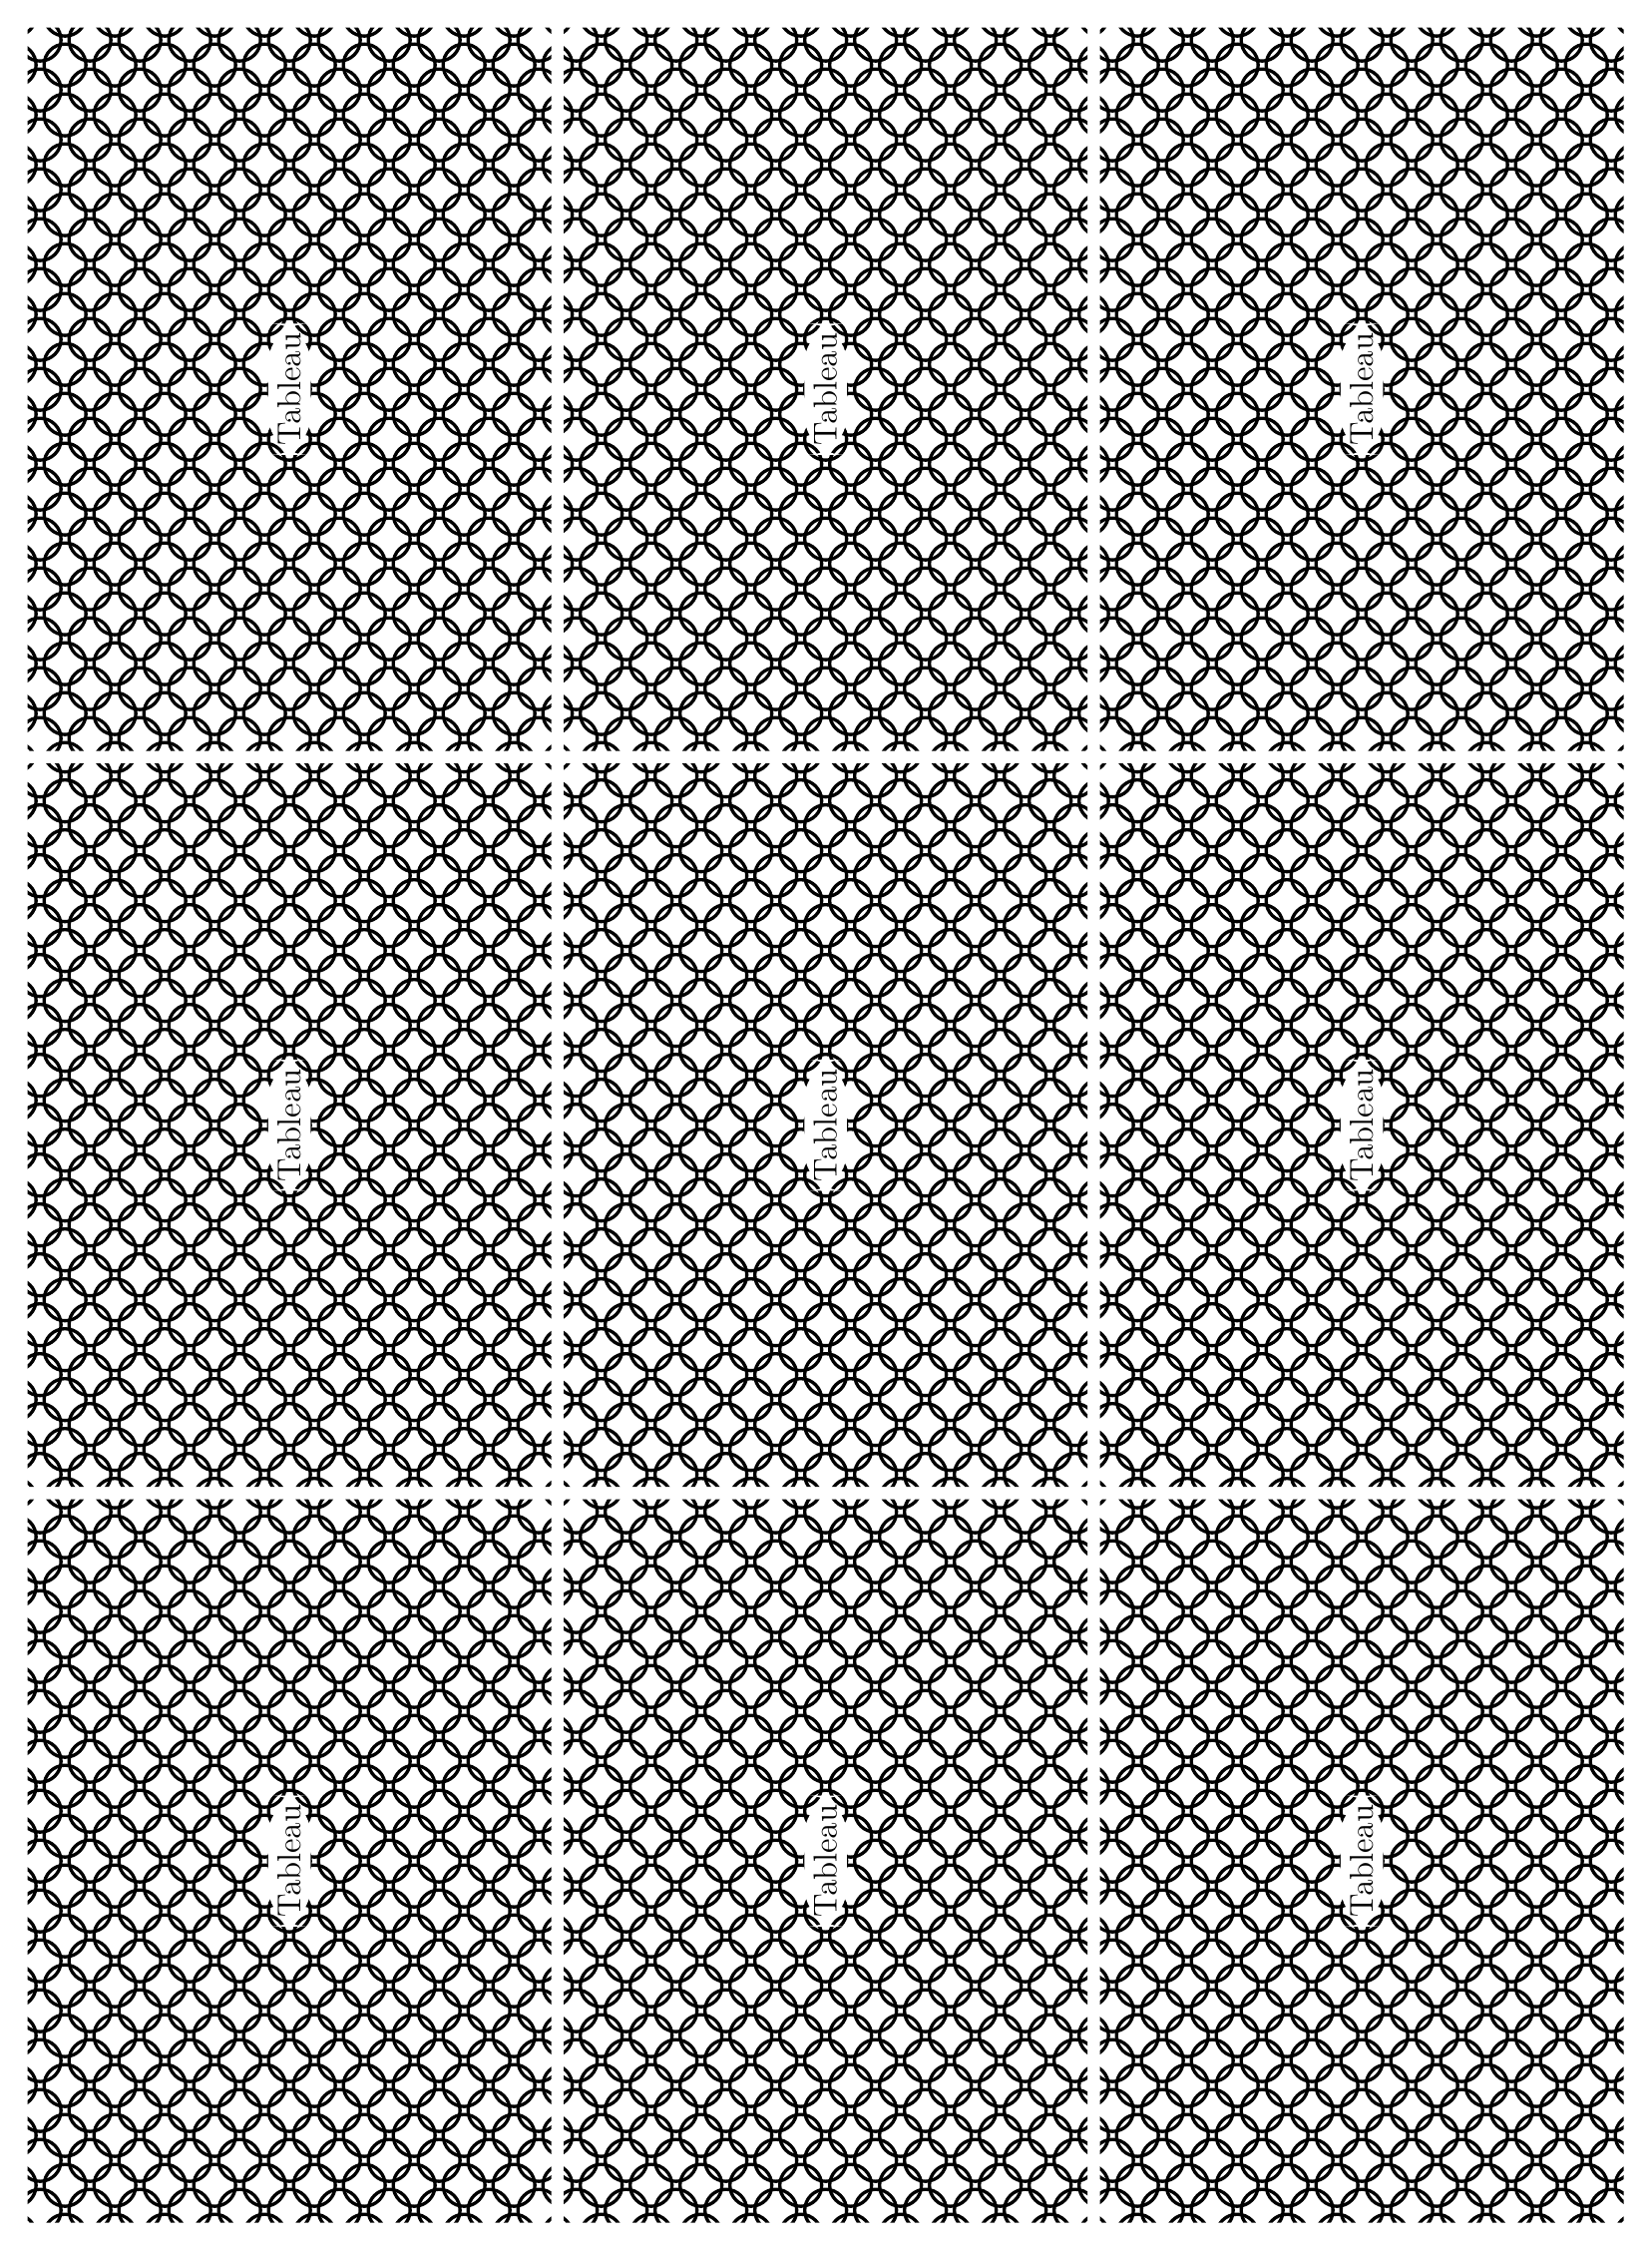
\begin{tikzpicture}[x=1in, y=1in]
\pic () at (0,0) {cardbackprintable={Tableau}};
\pic () at (\horizdist,0) {cardbackprintable={Tableau}};
\pic () at (2\horizdist,0) {cardbackprintable={Tableau}};

\pic () at (0,-\vertdist) {cardbackprintable={Tableau}};
\pic () at (\horizdist,-\vertdist) {cardbackprintable={Tableau}};
\pic () at (2\horizdist,-\vertdist) {cardbackprintable={Tableau}};

\pic () at (0,-2\vertdist) {cardbackprintable={Tableau}};
\pic () at (\horizdist,-2\vertdist) {cardbackprintable={Tableau}};
\pic () at (2\horizdist,-2\vertdist) {cardbackprintable={Tableau}};
\end{tikzpicture}	
\end{center}
\newpage
\setmainfont[Scale=1.0]{Cinzel}\phantom{a}\setmainfont[Scale=3.0]{Cinzel}
\begin{center}
\begin{tikzpicture}[x=1in, y=1in]
\pic () at (0,0) {tableaucardfrontprintable={dragon}};
\pic () at (\horizdist, 0) {tableaucardfrontprintable={dragon}};
\pic () at (2\horizdist, 0) {tableaucardfrontprintable={dragon}};

\pic () at (0, -\vertdist) {tableaucardfrontprintable={dragon}};
\pic () at (\horizdist, -\vertdist) {tableaucardfrontprintable={dragon}};
\pic () at (2\horizdist, -\vertdist) {tableaucardfrontprintable={dragon}};

\pic () at (0, -2\vertdist) {tableaucardfrontprintable={dragon}};
\pic () at (\horizdist, -2\vertdist) {tableaucardfrontprintable={dragon}};
\pic () at (2\horizdist, -2\vertdist) {tableaucardfrontprintable={dragon}};
\end{tikzpicture}	
\end{center}
\newpage
\setmainfont[Scale=1.0]{Cinzel}\phantom{a}\setmainfont[Scale=3.0]{Cinzel}
\begin{center}
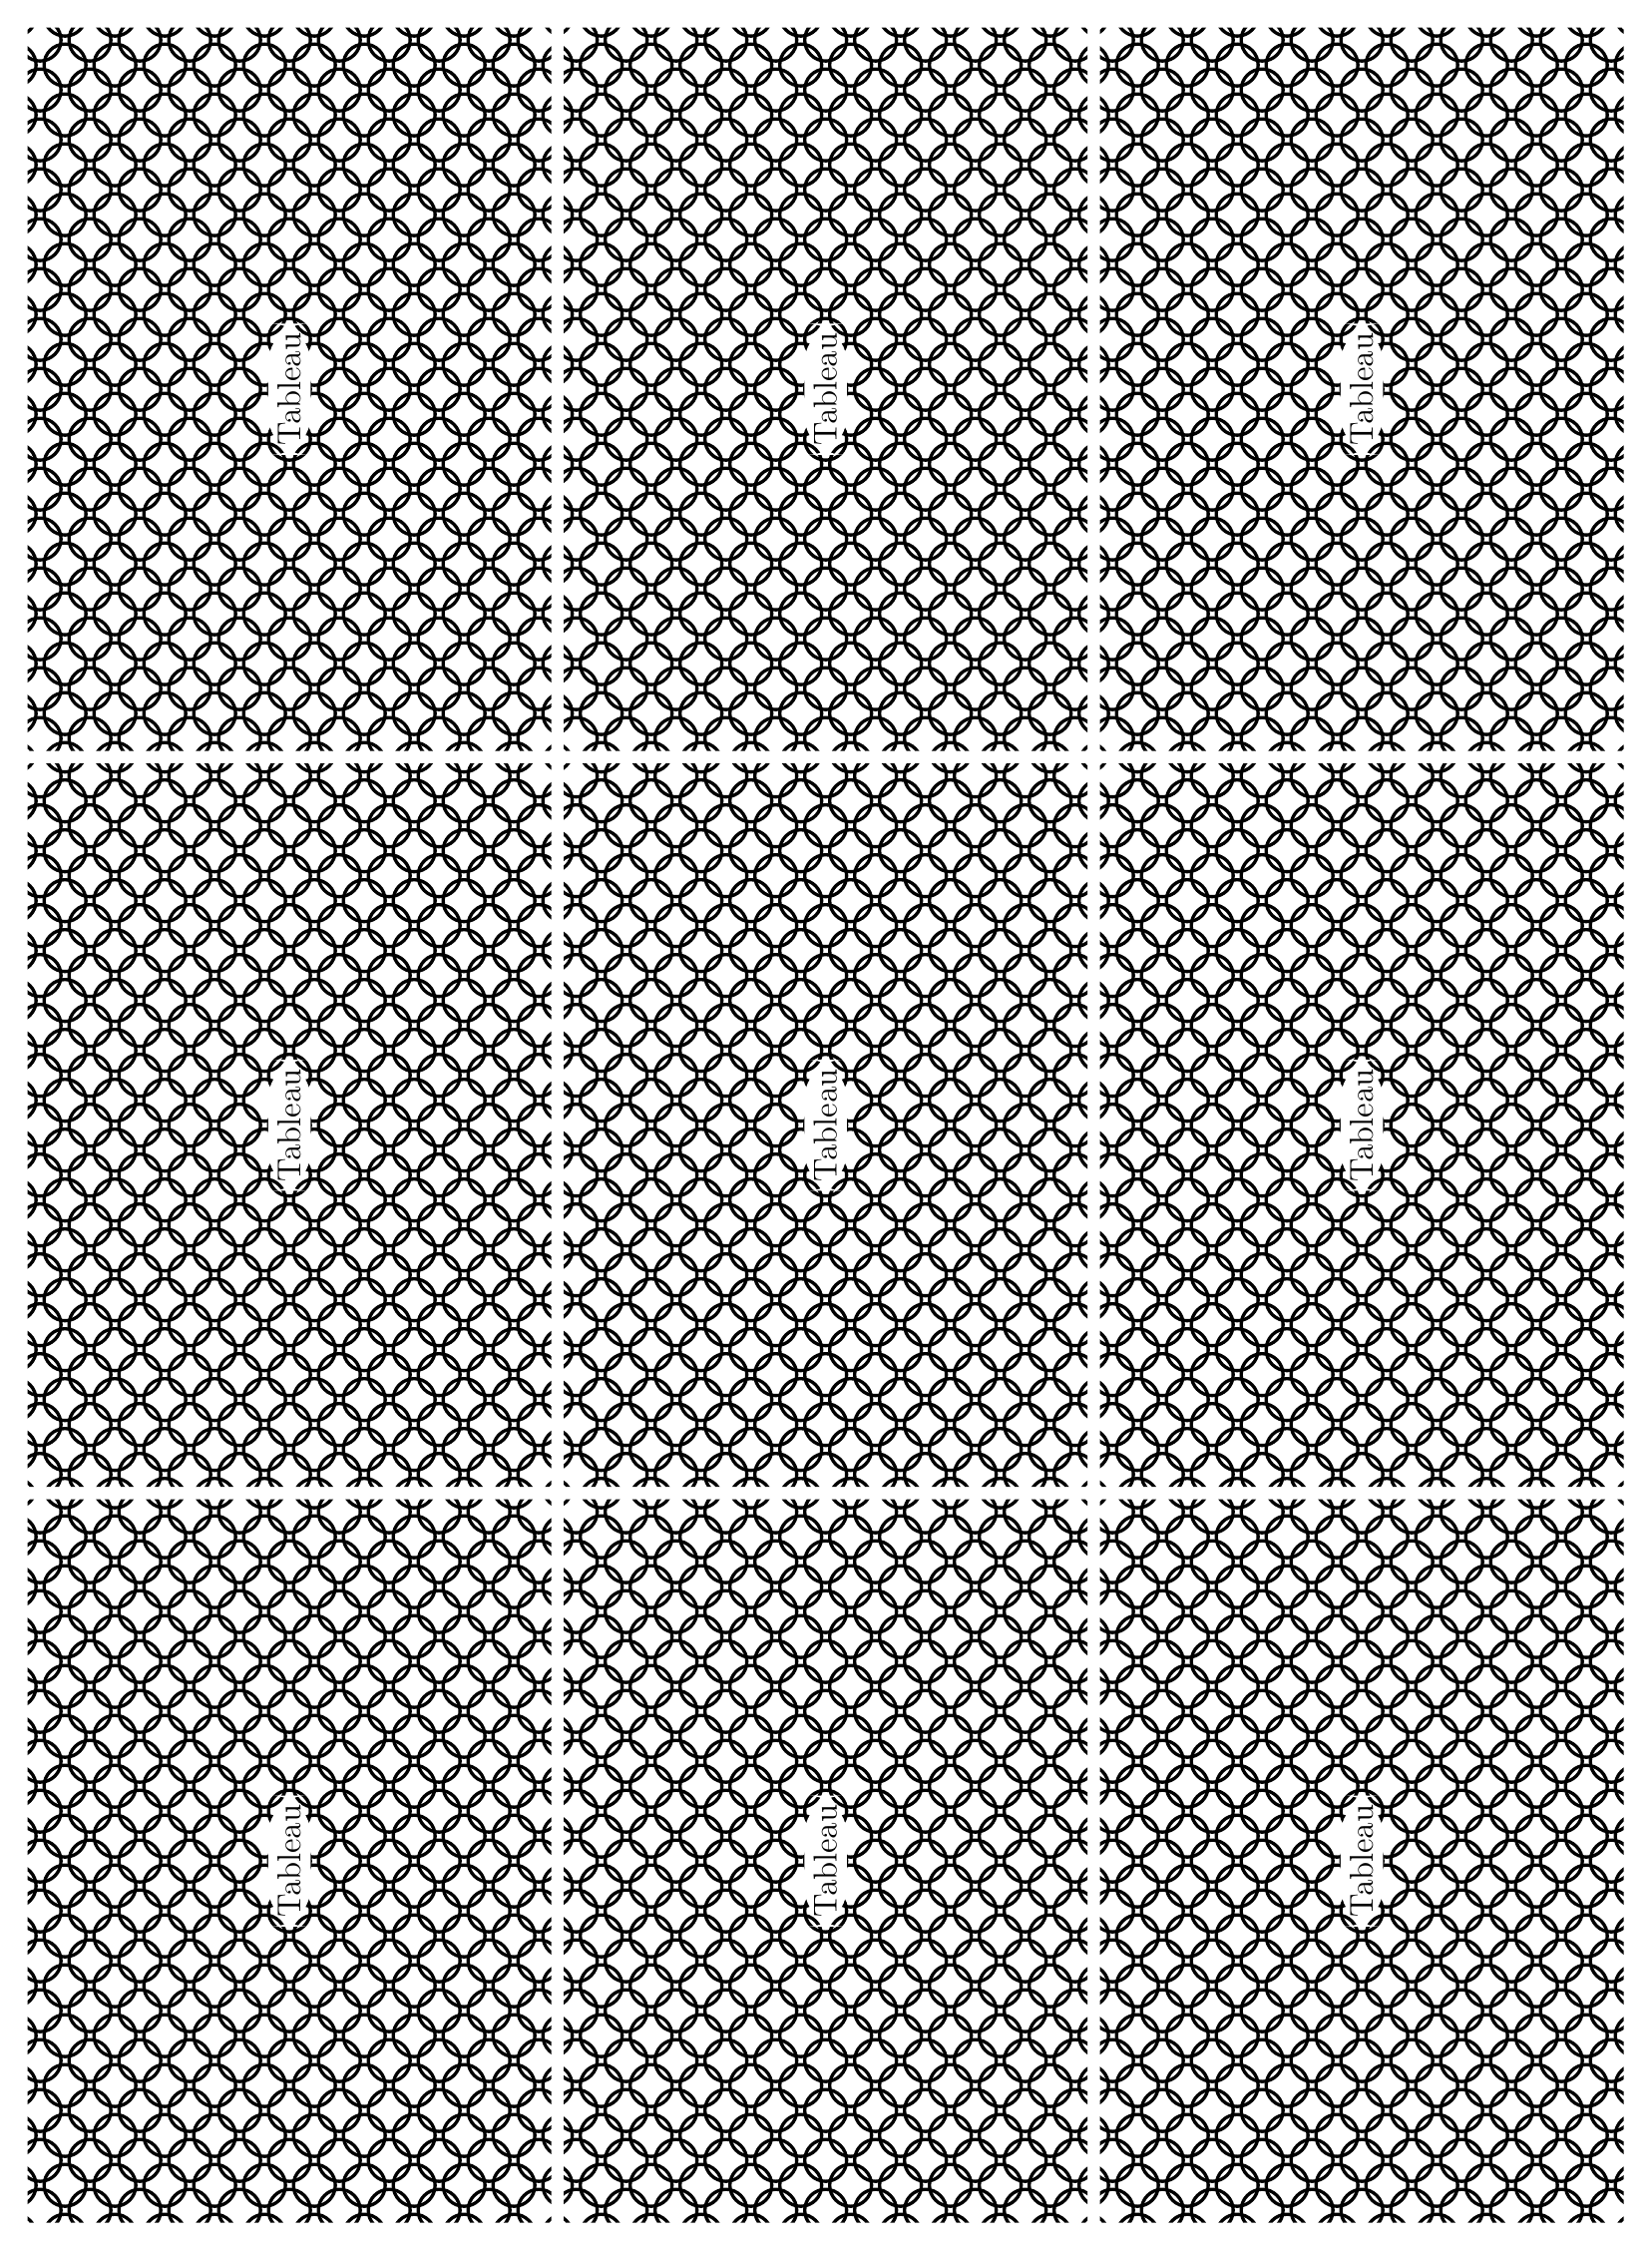
\begin{tikzpicture}[x=1in, y=1in]
\pic () at (0,0) {cardbackprintable={Tableau}};
\pic () at (\horizdist,0) {cardbackprintable={Tableau}};
\pic () at (2\horizdist,0) {cardbackprintable={Tableau}};

\pic () at (0,-\vertdist) {cardbackprintable={Tableau}};
\pic () at (\horizdist,-\vertdist) {cardbackprintable={Tableau}};
\pic () at (2\horizdist,-\vertdist) {cardbackprintable={Tableau}};

\pic () at (0,-2\vertdist) {cardbackprintable={Tableau}};
\pic () at (\horizdist,-2\vertdist) {cardbackprintable={Tableau}};
\pic () at (2\horizdist,-2\vertdist) {cardbackprintable={Tableau}};
\end{tikzpicture}	
\end{center}
\newpage
\setmainfont[Scale=1.0]{Cinzel}\phantom{a}\setmainfont[Scale=3.0]{Cinzel}
\begin{center}
\begin{tikzpicture}[x=1in, y=1in]
\pic () at (0,0) {tableaucardfrontprintable={eagle}};
\pic () at (\horizdist, 0) {tableaucardfrontprintable={eagle}};
\pic () at (2\horizdist, 0) {tableaucardfrontprintable={eagle}};

\pic () at (0, -\vertdist) {tableaucardfrontprintable={eagle}};
\pic () at (\horizdist, -\vertdist) {tableaucardfrontprintable={eagle}};
\pic () at (2\horizdist, -\vertdist) {tableaucardfrontprintable={eagle}};

\pic () at (0, -2\vertdist) {tableaucardfrontprintable={eagle}};
\pic () at (\horizdist, -2\vertdist) {tableaucardfrontprintable={eagle}};
\pic () at (2\horizdist, -2\vertdist) {tableaucardfrontprintable={eagle}};
\end{tikzpicture}	
\end{center}
\newpage
\setmainfont[Scale=1.0]{Cinzel}\phantom{a}\setmainfont[Scale=3.0]{Cinzel}
\begin{center}
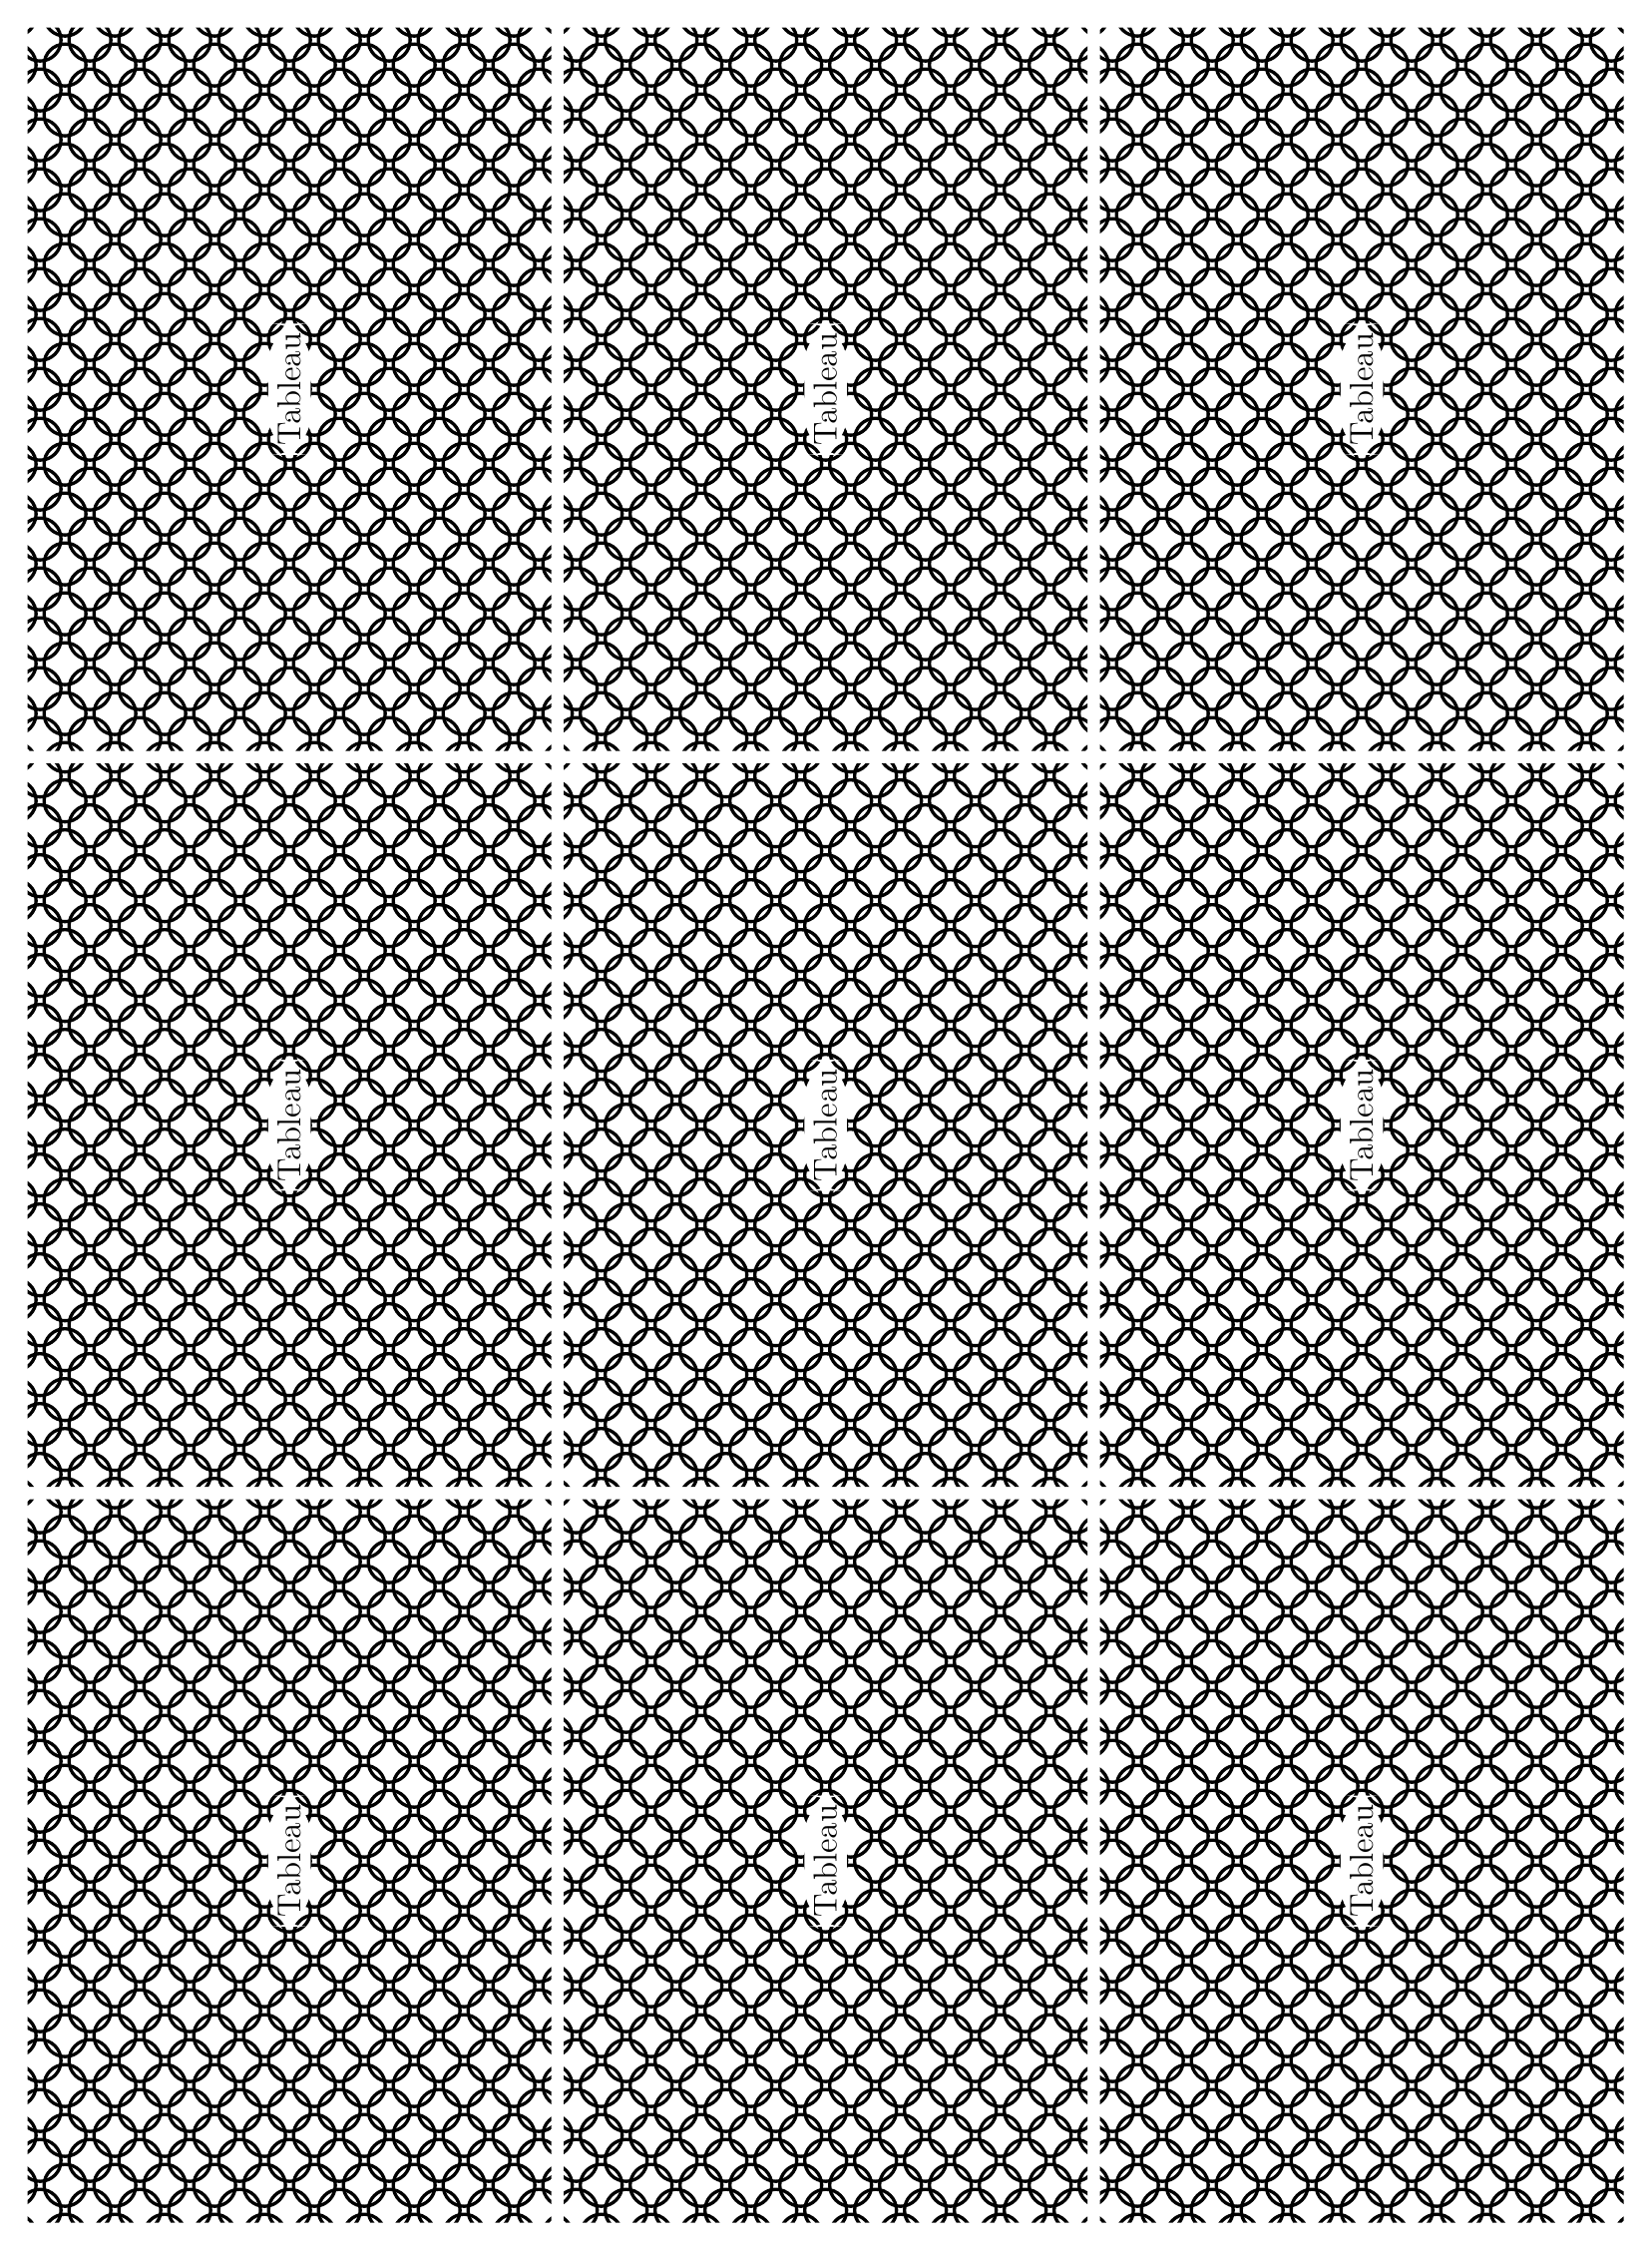
\begin{tikzpicture}[x=1in, y=1in]
\pic () at (0,0) {cardbackprintable={Tableau}};
\pic () at (\horizdist,0) {cardbackprintable={Tableau}};
\pic () at (2\horizdist,0) {cardbackprintable={Tableau}};

\pic () at (0,-\vertdist) {cardbackprintable={Tableau}};
\pic () at (\horizdist,-\vertdist) {cardbackprintable={Tableau}};
\pic () at (2\horizdist,-\vertdist) {cardbackprintable={Tableau}};

\pic () at (0,-2\vertdist) {cardbackprintable={Tableau}};
\pic () at (\horizdist,-2\vertdist) {cardbackprintable={Tableau}};
\pic () at (2\horizdist,-2\vertdist) {cardbackprintable={Tableau}};
\end{tikzpicture}	
\end{center}
\newpage
\setmainfont[Scale=1.0]{Cinzel}\phantom{a}\setmainfont[Scale=3.0]{Cinzel}
\begin{center}
\begin{tikzpicture}[x=1in, y=1in]
\pic () at (0,0) {tableaucardfrontprintable={wolf}};
\pic () at (\horizdist, 0) {tableaucardfrontprintable={wolf}};
\pic () at (2\horizdist, 0) {tableaucardfrontprintable={wolf}};

\pic () at (0, -\vertdist) {tableaucardfrontprintable={wolf}};
\pic () at (\horizdist, -\vertdist) {tableaucardfrontprintable={wolf}};
\pic () at (2\horizdist, -\vertdist) {tableaucardfrontprintable={wolf}};

\pic () at (0, -2\vertdist) {tableaucardfrontprintable={wolf}};
\pic () at (\horizdist, -2\vertdist) {tableaucardfrontprintable={wolf}};
\pic () at (2\horizdist, -2\vertdist) {tableaucardfrontprintable={wolf}};
\end{tikzpicture}	
\end{center}
\end{document}